\documentclass[a4paper]{article}
\usepackage[pdftex]{hyperref}
\usepackage[latin1]{inputenc}
\usepackage[english]{babel}
\usepackage{a4wide}
\usepackage{array}
\usepackage{tabu}
\usepackage{amsmath}
\usepackage{amssymb}
\usepackage{setspace}
\usepackage{algorithmic}
\usepackage{algorithm}
\usepackage{ifthen}
\usepackage{listings}
% move the asterisk at the right position
\lstset{basicstyle=\ttfamily,tabsize=4,literate={*}{${}^*{}$}1}
%\lstset{language=C,basicstyle=\ttfamily}
\usepackage{moreverb}
\usepackage{palatino}
\usepackage{multicol}
\usepackage{tabularx}
\usepackage{comment}
\usepackage{verbatim}
\usepackage{color}
\usepackage{graphicx}
\graphicspath{ {/Users/fjolladedaj/Desktop/2nd\ Year/Computer\ Architecture\ and\ Programming\ Languages/HW_2/Solution} }

%% pdflatex?
\newif\ifpdf
\ifx\pdfoutput\undefined
\pdffalse % we are not running PDFLaTeX
\else
\pdfoutput=1 % we are running PDFLaTeX
\pdftrue
\fi
\ifpdf
\usepackage{graphicx}
\else
\usepackage{graphicx}
\fi
\ifpdf
\DeclareGraphicsExtensions{.pdf, .jpg}
\else
\DeclareGraphicsExtensions{.eps, .jpg}
\fi

\parindent=0cm
\parskip=0cm

\setlength{\columnseprule}{0.4pt}
\addtolength{\columnsep}{2pt}

\addtolength{\textheight}{5.5cm}
\addtolength{\topmargin}{-26mm}
\pagestyle{empty}

%%
%% Sheet setup
%% 
\newcommand{\coursename}{Computer Architecture and Programming Languages}
\newcommand{\courseno}{CO20-320241}
 
\newcommand{\sheettitle}{Homework}
\newcommand{\mytitle}{}
\newcommand{\mytoday}{{September 23}, 2019}

% Current Assignment number
\newcounter{assignmentno}
\setcounter{assignmentno}{2}

% Current Problem number, should always start at 1
\newcounter{problemno}
\setcounter{problemno}{1}

%%
%% problem and bonus environment
%%
\newcounter{probcalc}
\newcommand{\problem}[2]{
  \pagebreak[2]
  \setcounter{probcalc}{#2}
  ~\\
  {\large \textbf{Problem \textcolor{blue}{\arabic{assignmentno}}.\textcolor{blue}{\arabic{problemno}}} \hspace{0.2cm}\textit{#1}} \refstepcounter{problemno}\vspace{2pt}\\}

\newcommand{\bonus}[2]{
  \pagebreak[2]
  \setcounter{probcalc}{#2}
  ~\\
  {\large \textbf{Bonus Problem \textcolor{blue}{\arabic{assignmentno}}.\textcolor{blue}{\arabic{problemno}}} \hspace{0.2cm}\textit{#1}} \refstepcounter{problemno}\vspace{2pt}\\}

%% some counters  
\newcommand{\assignment}{\arabic{assignmentno}}

%% solution  
\newcommand{\solution}{\pagebreak[2]{\bf Solution:}\\}

%% Hyperref Setup
\hypersetup{pdftitle={Homework \assignment},
  pdfsubject={\coursename},
  pdfauthor={},
  pdfcreator={},
  pdfkeywords={Computer Architecture and Programming Languages},
  %  pdfpagemode={FullScreen},
  %colorlinks=true,
  %bookmarks=true,
  %hyperindex=true,
  bookmarksopen=false,
  bookmarksnumbered=true,
  breaklinks=true,
  %urlcolor=darkblue
  urlbordercolor={0 0 0.7}
}

\begin{document}
\coursename \hfill Course: \courseno\\
Jacobs University Bremen \hfill \mytoday\\
{Fjolla Dedaj}\hfill
\vspace*{0.3cm}\\
\begin{center}
{\Large \sheettitle{} \textcolor{blue}{\assignment}\\}
\end{center}

\problem{}{0}
\solution
\\
\textbf{a)} $777_8 + 1_8 = \mathbf{1000_8}$\\
\\
\textbf{b)} $888_16 + 1_{16} = \mathbf{889_{16}}$\\
\\
\textbf{c)} $32007_8 + 1_8 = \mathbf{32010_{8}}$\\
\\
\textbf{d)} $32108_{16} + 1_{16} = \mathbf{32109_{16}}$\\
\\
\textbf{e)} $8BFF_{16} + 1_{16} = \mathbf{8C00_{16}}$\\
\\
\textbf{f)} $1219_{16} + 1_{16} = \mathbf{121A_{16}}$\\
\\
\problem{}{0}
\solution
\\
\textbf{a)} $X = \overline{A*B*(C+D)}$ \\ 
\\
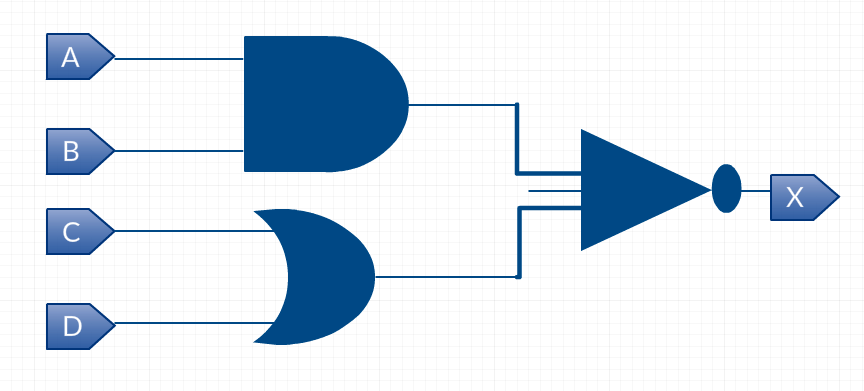
\includegraphics[scale=0.3]{circuit1.png}\\
\\
\textbf{b)} $X = \overline{A+B+\overline{C}*D*\overline{E}}+ \overline{B} + C + \overline{D}$\\
\\ 
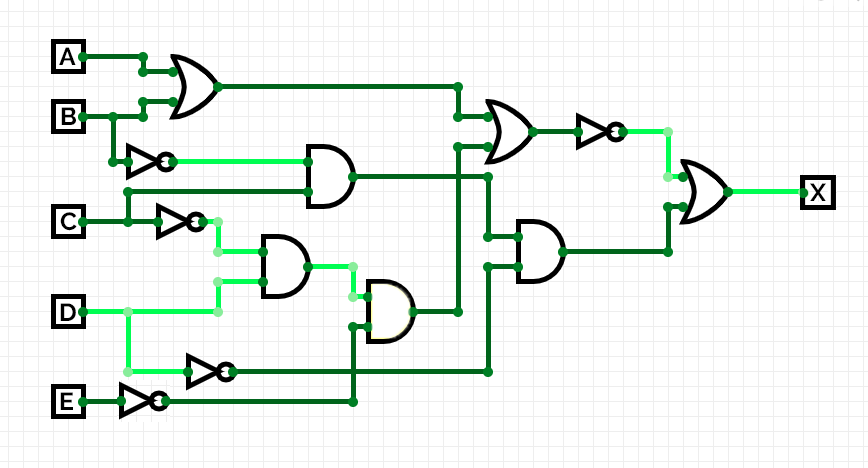
\includegraphics[scale=0.3]{circuit2.png}\\
\\
\textbf{c)}\\ 
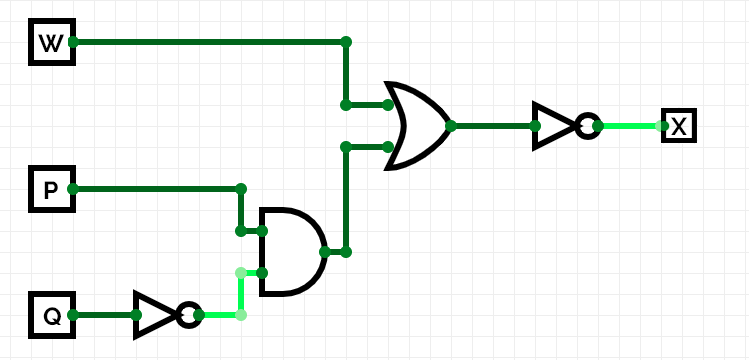
\includegraphics[scale=0.3]{circuit3.png}\\
\\
\textbf{d)}\\ 
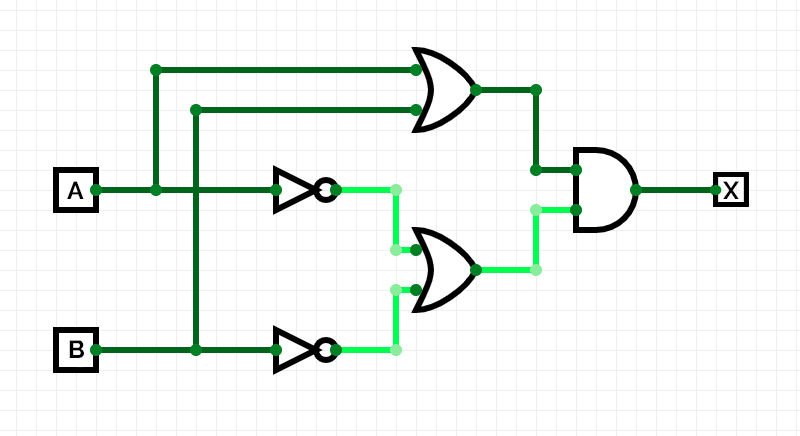
\includegraphics[scale=0.3]{circuit4.png}\\
\\

\problem{}{0}
\solution
\\
$R1 = \overline{M * N * Q}\\
R2 =\overline{M * \overline{N} * Q}\\
R3 = \overline{\overline{M} * N * Q}$
\\
\\
The truth table of the circuit:
\\
\begin{tabu} to 0.8\textwidth { | X[c] | X[c] | X[c] | X[c] | X[c] | X[c] | X[c] | }
 \hline
 M & N  & Q & R1 & R2 & R3 & X  \\
 \hline
 $0$  & $0$  & $0$  & $1$ & $1$ & $1$  & $0$\\
 \hline
 $0$  & $0$  & $1$ & $1$ & $1$ & $1$  & $0$\\
 \hline
 $0$  & $1$  & $0$ & $1$ & $1$ & $1$  & $0$\\
 \hline
 $0$  & $1$  & $1$ & $1$ & $1$ & $0$  & $1$\\
 \hline
 $1$  & $0$  & $0$  & $1$ & $1$ & $1$  & $0$\\
 \hline
 $1$  & $0$  & $1$ & $1$ & $0$ & $1$  & $1$\\
 \hline
 $1$  & $1$  & $0$ & $1$ & $1$ & $1$  & $0$\\
 \hline
 $1$  & $1$  & $1$ & $0$ & $1$ & $1$  & $1$\\
\hline
\end{tabu}
\\
\\
The sum of products:
$X = \overline{M} * N * Q + M * \overline{N} * Q + M * N * Q$
\\
\\
Simplify:\\
$X = \overline{M} * N * Q + M * \overline{N} * Q + M * N * Q =\\
Distributive$ $Law: = Q(\overline{M} * N + M * \overline{N} + M * N) = \\ 
Distributive$ $Law: = Q(\overline{M} * N + M * \overline{N} + M * N + M * N) = \\ 
Distributive$ $Law: = Q(N(\overline{M} + M) + M(\overline{N} + N)) = \\ 
Identity$ $Law: = Q(N * 1 + M * 1) = \\ 
Distributive$ $Law: = Q(N + M) = Q * N + Q * M\\$
\\
Circuit Representation after simplification:
\\
\\
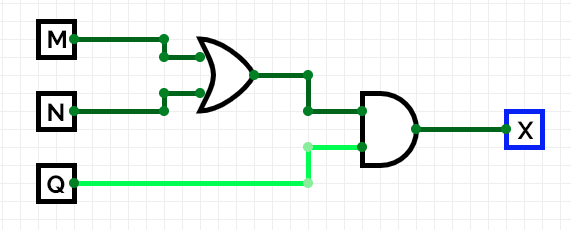
\includegraphics[scale=0.3]{circuit5.png}\\
\\
\pagebreak
\problem{}{0}
\solution
\\
\textbf{a)}\\ 
$X + \overline{X}*{Y} = X + {Y}$
\\
\\
$X + \overline{X}*{Y}$:
\\
\begin{tabu} to 0.8\textwidth { | X[c] | X[c] | X[c] | X[c] | X[c] | }
 \hline
 X & Y  & $\overline{X}$ & $\overline{X}\wedge Y$ & $ X \vee ( \overline{X} \wedge{Y}) $  \\
 \hline
 $0$  & $0$  & $1$  & $0$ & $0$\\
 \hline
 $0$  & $1$  & $1$ & $1$ & $1$\\
 \hline
 $1$  & $0$  & $0$ & $0$ & $1$\\
 \hline
 $1$  & $1$  & $0$ & $0$ & $1$\\
\hline
\end{tabu}
\\
\\
\\
$X + {Y}$:
\\
\begin{tabu} to 0.8\textwidth { | X[c] | X[c] | X[c] | }
 \hline
 X & Y  & $ X \vee Y $\\
 \hline
 $0$  & $0$  & $0$\\
 \hline
 $0$  & $1$  & $1$\\
 \hline
 $1$  & $0$  & $1$\\
 \hline
 $1$  & $1$  & $1$\\
\hline
\end{tabu}
\\
\\
As it is evident, both sides of the equation result in the same output.
\\
\\
\textbf{b)}\\ 
$\overline{X} + X * Y = \overline{X} + Y$
\\
\\
$\overline{X} + X * Y$:
\\
\begin{tabu} to 0.8\textwidth { | X[c] | X[c] | X[c] | X[c] | X[c] | }
 \hline
 X & Y  & $\overline{X}$ & $X \wedge Y$ & $ \overline{X} \vee ( X \wedge{Y}) $  \\
 \hline
 $0$  & $0$  & $1$  & $0$ & $1$\\
 \hline
 $0$  & $1$  & $1$ & $0$ & $1$\\
 \hline
 $1$  & $0$  & $0$ & $0$ & $0$\\
 \hline
 $1$  & $1$  & $0$ & $1$ & $1$\\
\hline
\end{tabu}
\\
\\
\\
$\overline{X} + Y$:
\\
\begin{tabu} to 0.8\textwidth { | X[c] | X[c] | X[c] | X[c] | }
 \hline
 X & Y  & $\overline{X}$ & $ \overline{X} \vee Y $\\
 \hline
 $0$  & $0$  & $1$ & $1$\\
 \hline
 $0$  & $1$  & $1$ & $1$\\
 \hline
 $1$  & $0$  & $0$ & $0$\\
 \hline
 $1$  & $1$  & $0$ & $1$\\
\hline
\end{tabu}
\\
\\
As it is evident, both sides of the equation result in the same output.
\\
\problem{}{0}
\solution
\\
\textbf{a)} $A + 1 = 1$
\\
\\
\textbf{b)} $A * A = A$
\\
\\
\textbf{c)} $B * \overline{B} = 0$
\\
\\
\textbf{d)} $C + C = C$
\\
\\
\textbf{e)} $X * 0 = 0$
\\
\\
\textbf{f)} $D * 1 = D$
\\
\\
\textbf{g)} $D + 0 = D$
\\
\\
\textbf{h)} $C + \overline{C} = 1$
\\
\\
\textbf{i)} $G + G * F = G$
\\
\\
\textbf{j)} $Y + \overline{W} * Y = Y$
\\
\\
\pagebreak
\problem{}{0}
\solution
\\
\textbf{1.} $\overline{W + Y} = \overline{W} * \overline{Y}$ \\
\\
\begin{tabu} to 0.8\textwidth { | X[c] | X[c] | X[c] | X[c] | X[c] | X[c] | X[c] | }
 \hline
 $W$ & $Y$  & $\overline{W}$ & $ \overline{Y}$ & $W + Y$ & $\overline{W+Y}$ & $\overline{W} \wedge \overline{Y}$\\
 \hline
 $0$  & $0$  & $1$ & $1$ & $0$ & $\textbf{1}$ & $\textbf{1}$\\
 \hline
 $0$  & $1$  & $1$ & $0$ & $1$ & $\textbf{0}$ & $\textbf{0}$\\
 \hline
 $1$  & $0$  & $0$ & $1$ & $1$ & $\textbf{0}$ & $\textbf{0}$\\
 \hline
 $1$  & $1$  & $0$ & $0$ & $1$ & $\textbf{0}$ & $\textbf{0}$\\
\hline
\end{tabu}
\\
\\
\\
\textbf{2.} $\overline{W * Y} = \overline{W} + \overline{Y}$ \\
\\
\begin{tabu} to 0.8\textwidth { | X[c] | X[c] | X[c] | X[c] | X[c] | X[c] | X[c] | }
 \hline
 $W$ & $Y$  & $\overline{W}$ & $ \overline{Y}$ & $W * Y$ & $\overline{W * Y}$ & $\overline{W} + \overline{Y}$\\
 \hline
 $0$  & $0$  & $1$ & $1$ & $0$ & $\textbf{1}$ & $\textbf{1}$\\
 \hline
 $0$  & $1$  & $1$ & $0$ & $0$ & $\textbf{1}$ & $\textbf{1}$\\
 \hline
 $1$  & $0$  & $0$ & $1$ & $0$ & $\textbf{1}$ & $\textbf{1}$\\
 \hline
 $1$  & $1$  & $0$ & $0$ & $1$ & $\textbf{0}$ & $\textbf{0}$\\
\hline
\end{tabu}
\\
\\
\\
\textbf{3.} $1 + W = 1$ \\
\\
\begin{tabu} to 0.8\textwidth { | X[c] | X[c] | X[c] | }
 \hline
 $1$ & $W$  & $1 \vee W$\\
 \hline
 $1$  & $0$  & $1$\\
 \hline
 $1$  & $0$  & $1$\\
 \hline
 $1$  & $1$  & $1$\\
 \hline
 $1$  & $1$  & $1$\\
\hline
\end{tabu}
\\
\\
\\
\textbf{4.} $0 + W = W$ \\
\\
\begin{tabu} to 0.8\textwidth { | X[c] | X[c] | X[c] | }
 \hline
 $0$ & $W$  & $1 \vee W$\\
 \hline
 $0$  & $0$  & $0$\\
 \hline
 $0$  & $0$  & $0$\\
 \hline
 $0$  & $1$  & $1$\\
 \hline
 $0$  & $1$  & $1$\\
\hline
\end{tabu}
\\
\\
\\
\textbf{5.} $0 * W = 0$ \\
\\
\begin{tabu} to 0.8\textwidth { | X[c] | X[c] | X[c] | }
 \hline
 $0$ & $W$  & $0 \wedge W$\\
 \hline
 $0$  & $0$  & $0$\\
 \hline
 $0$  & $0$  & $0$\\
 \hline
 $0$  & $1$  & $0$\\
 \hline
 $0$  & $1$  & $0$\\
\hline
\end{tabu}
\\
\\
\\
\textbf{6.} $1 * W = W$ \\
\\
\begin{tabu} to 0.8\textwidth { | X[c] | X[c] | X[c] | }
 \hline
 $1$ & $W$  & $1 \wedge W$\\
 \hline
 $1$  & $0$  & $0$\\
 \hline
 $1$  & $0$  & $0$\\
 \hline
 $1$  & $1$  & $1$\\
 \hline
 $1$  & $1$  & $1$\\
\hline
\end{tabu}
\\
\\
\pagebreak
\problem{}{0}
\\
DL = Distributive Law\\
CL = Complement Law\\
IL = Identity Law\\
\\
The sum-of-product expression: \\
\\
$X = \overline{A} * \overline{B} * \overline{C} * D + \overline{A} * \overline{B} * C * D + \overline{A} * B * \overline{C} * D + \overline{A} * B * C * D + A * \overline{B} * \overline{C} * \overline{D} + A * B * \overline{C} * D + A * B * C * D =  \\
\\
DL: = A * \overline{B} * \overline{C} * \overline{D} + D(\overline{A} * \overline{B} * \overline{C} + \overline{A} * \overline{B} * C + \overline{A} * B * \overline{C} + \overline{A} * B * C + A * B * \overline{C} + A * B * C) = \\
\\
DL: = A * \overline{B} * \overline{C} * \overline{D} + D(\overline{A} * \overline{B} * (\overline{C} * C) + \overline{A}*B*(\overline{C} + C) + A * B * (\overline{C} + C)) = \\
\\
CL: = A * \overline{B} * \overline{C} * \overline{D} + D(\overline{A} * \overline{B} * 1 + \overline{A}*B*1 + A * B * 1) =\\
\\
IL: = A * \overline{B} * \overline{C} * \overline{D} + D(\overline{A} * \overline{B} + \overline{A}*B + A * B)\\
\\
$Since $ A + A = A, $ write $ \overline{A} * B = \overline{A}*B + \overline{A} * B:\\
\\
X = A * \overline{B} * \overline{C} * \overline{D} + D(\overline{A} * \overline{B} + \overline{A}*B + \overline{A}*B + A * B) =\\
\\
DL: = A * \overline{B} * \overline{C} * \overline{D} + D(\overline{A} * (\overline{B} + B) + B*(\overline{A} + A)) =\\
\\
CL: = A * \overline{B} * \overline{C} * \overline{D} + D(\overline{A} * 1 + B*1) =\\
\\
IL: = A * \overline{B} * \overline{C} * \overline{D} + D(\overline{A} + B) =\\
\\
DL: = A * \overline{B} * \overline{C} * \overline{D} + \overline{A} * D + B*D\\
\\
$
\problem{}{0}
\solution
\\
\\
\begin{tabu} to 0.8\textwidth {  X[c] | X[c] | X[c] | X[c] | X[c] | }
 $ $ & $\overline{C}\overline{D}$ & $\overline{C}D$ & $CD$ & $C\overline{D}$ \\
 \hline
  $\overline{A}\overline{B}$ & $0$  & \textcolor{blue}{$1$} & \textcolor{blue}{$1$}  & $0$\\
 \hline
  $\overline{A}B$  & $0$  & \textcolor{blue}{$1$} $\wedge$ \textcolor{red}{$1$} & \textcolor{blue}{$1$} $\wedge$ \textcolor{red}{$1$} & $0$\\
 \hline
 $AB$  & $0$  & \textcolor{red}{$1$} & \textcolor{red}{$1$}  & $0$\\
 \hline
 $A\overline{B}$ & \textcolor{green}{$1$}  & $0$ & $0$  & $0$\\
\hline
\end{tabu}
\\
\\
\\
$Note$: the 1s in the second row belong to both groups (red 1s and blue 1s) in order to give the minimalistic expression.
\\
\\
After building the Karnaugh-map using gray coding (00, 01, 11, 10) from the truth table given in \textbf{Problem 2.7}, we first try to create groups of 1s.
We have 3 groups in total, distinguished by their colors (red, blue and green).\\
Green group (single 1): all terms are included $=>$ $A * \overline{B} * \overline{C} * \overline{D}$.\\
Blue group: $\overline{A} * D =>$ These terms do not change regardless of the output.\\
Red group: similarly $=> B * D$\\
As a result, we obtain: $\mathbf{X = A * \overline{B} * \overline{C} * \overline{D} + \overline{A} * D + B * D} $\\
\end{document}

 